\documentclass[10pt,a4paper]{article}
\usepackage[utf8]{inputenc}
\usepackage[english]{babel}
\usepackage{amsmath}
\usepackage{amsfonts}
\usepackage{amssymb}
\usepackage{graphicx}
\usepackage[left=4cm,right=4cm,top=4cm,bottom=4cm]{geometry}
\usepackage{natbib}

\renewcommand{\vec}[1]{\mathbf{#1}}

\newcommand{\vx}{\vec{x}}
\newcommand{\vy}{\vec{y}}
\newcommand{\vf}{\vec{f}}
\newcommand{\vsigm}{\boldsymbol{\sigma}}

\newcommand{\Err}{\mathrm{Err}}
\newcommand{\Exp}{\mathrm{E}}
\newcommand{\Var}{\mathrm{Var}}

\newcommand{\avg}[1]{\langle #1 \rangle}

\newcommand{\Wout}{\hat{\mathrm{W}}_{\rm out}}
\newcommand{\Win}{\hat{\mathrm{W}}_{\rm in}}
\newcommand{\Wrec}{\hat{\mathrm{W}}}

\author{Fabian Schubert}

\title{Learning in a Simplified Neural Compartment Model}

\usepackage{layouts}

\begin{document}
\maketitle

%\section{Introduction}
%
%
%How can a dynamical system with states $\vx(t)$ be modified appropriately, such that it can generate an output signal $\vy(t)$ that mimics or predicts some target signal $\vf(t)$?
%
%One variant of this task consists of training $\vx(t)$ to autonomously generate an output $\vy(t)$ that equals $\vf(t)$.\\
%The other task, which we shall focus on, includes feeding the signal $\vf(t)$ into the dynamical system which is the supposed to generate an output $\vy(t)$ that correctly predicts $\vf(t+1)$.
%
%Formally, the goal of such a temporal prediction task is to find a function $\vy(\cdot)$
%\begin{equation}
%\vy(t) = \vy\left( \vf(t),\vf(t-1),\vf(t-2),...\right)
%\end{equation}
%such that it minimizes an error measure, typically the RMS
%\begin{equation}
%\Err\left(\vf(t),\vy(t)\right) = \frac{\sqrt{\left| \vf(t) - \vy(t)\right|^2}}{\Var\left[ | \vf|\right]} \; .
%\end{equation}
%
%The general idea of how to approach this is to expand the sequence $\left\{ \vf(t-1),\vf(t-2), ...\right\}$ into some high-dimensional feature vector $\vx(t)$ which is then used to predict $\vf(t)$ by a linear model
%\begin{equation}
%\vy(t) = \Wout \vx(t) = \Wout \vx\left( \vf(t-1),\vf(t-2),...\right) \;
%\end{equation}
%This expansion has a potentially unbounded amount of parameters, so one takes a recursive approach:
%\begin{equation}
%\vx(t) = \vx\left(\vx(t-1),\vf(t-1)\right) \;.
%\end{equation}
%We can further restrict this form to recursive functions that take the form of a discrete-time recurrent network:
%\begin{equation}
%\vx(t) = \vsigm \left( \Wrec \vx (t-1) + \Win \vf(t-1) \right) \; .
%\end{equation}
%
%Recurrent networks for sequence learning have been extensively studied in the field of machine learning \cite{Rumelhart_1988,Elman_1990}. Generally speaking, a recurrent network serves as a reservoir for storing information about the past of an input stream. In classical machine learning approaches, the sequence learning task is a problem of appropriately setting the linear components of the recursive function as well as of the readout to minimize the error.
%
%\section{Backpropagation Through Time}
%The idea of the BPTT algorithm is to unfold recurrent causal relations in the network into a feed-forward network structure, which can then be learned with a normal backpropagation algorithm, see Fig. \ref{fig:BPTT}.
%\begin{figure}
%\centering
%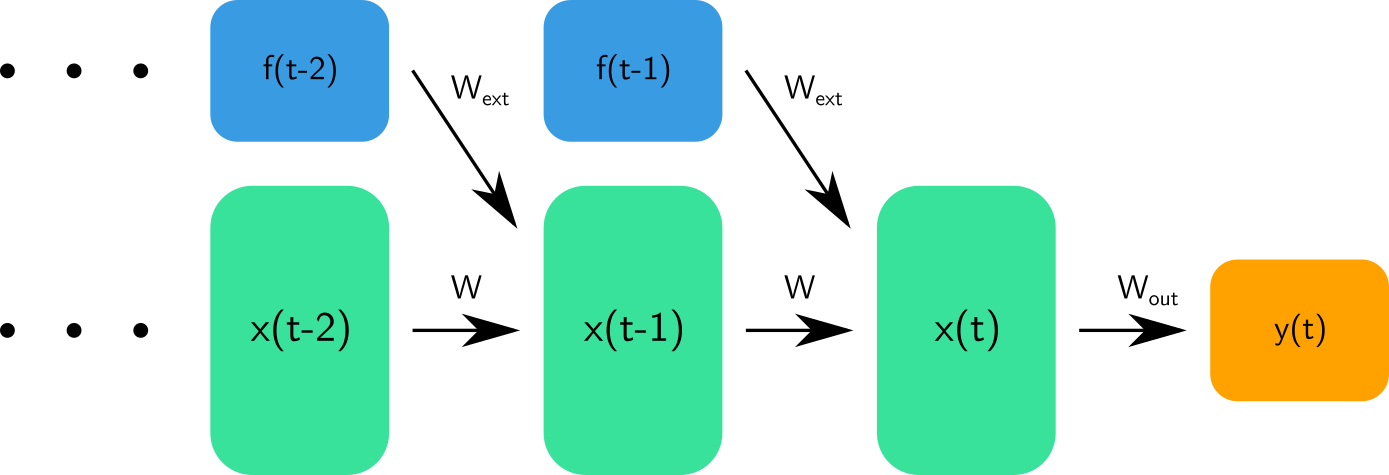
\includegraphics[width=0.6\textwidth]{./figures/backpropagation_through_time.png}
%\caption{Illustration of the BPTT algorithm.}
%\label{fig:BPTT}
%\end{figure}
%
%\subsection{Possible Mechanism of Sequence Learning in the Brain}
%
%Models of error-driven sequence learning have been studied quite extensively, including simple recurrent networks \cite{Elman_1990,Jordan_1989}, as well as the more recent approach of using a Bayesian learning framework to create a generative model of the environment \cite{Friston_2005}. A critical aspect of a predictive framework is that it requires some form of time discretization in order to clearly separate ``future" states or inputs to be predicted from current states. It has been argued that alpha rhythm arising from thalamic neurons might define the pace of such a perceptual and predictive discretization \cite{OReilly_2014}.
%
%Since predictive learning has to be error-driven in some sense, it requires a plasticity mechanism reflecting this requirement. We propose dendritic coincidence detection, gating synaptic plasticity for this purpose. It has been shown that distally evoked dendritic potentials can control plasticity at other synapses \cite{Clopath_Bono_2017}, which fits to the results of the simulations we performed for a single neuron based on a model proposed by Shai et al. \cite{Shai_2015}.
%
%\section{Echo-State Networks}
%
%More recently, so-called echo-state networks have been used in sequence learning \cite{Jaeger_2010}. Instead of training the input, recurrent and output weights, only the readout weights are trained in this framework. A recurrent neural network is randomly created and remains unchanged during training. It needs to contain a large number of nodes ($\sim 10^2 - 10^3$), have a random connectivity structure and must be sparse. The ``echo state property" states that the effect of external input on the internal state should vanish gradually over time.
%
%This architecture is more biologically plausible, since the details of the reservoir are not important, and access to the error is only required for the readout units. Still, the readout needs access to the input signal for comparison, and it is not clear how this could be implemented biologically. Furthermore, readout weights are usually trained via gradient descent of the error, which is not biologically motivated. Ideally, we would like to use an Hebbian type learning rule to learn the readout, while providing some direct access to the input signal to predict.

\section{Dendritic Computation for Sequence Prediction}

%\printinunitsof{in}\prntlen{\textwidth}

Shai et al. proposed a phenomenological model describing neural activity as a function of basal and distal synaptic input in pyramidal neurons \cite{Shai_2015}, see Fig. \ref{fig:Shai_prox_dist}.
\begin{figure}
\centering
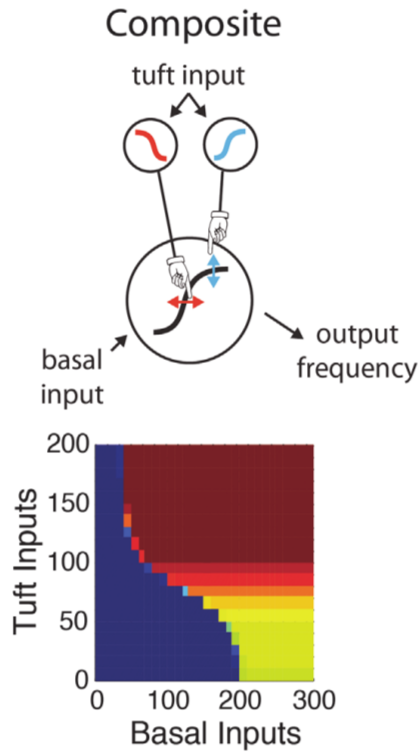
\includegraphics[width=0.3\textwidth]{./figures/shai_phen_model.png}
\caption{Firing rate as a function of distal and proximal input of the rate model proposed in \cite{Shai_2015}.}
\label{fig:Shai_prox_dist}
\end{figure}
We further simplified this model to the following form:
\begin{align}
y\left(I_p,I_d\right) &= \sigma\left(I_p-\theta^{\rm p}_{1}\right) \sigma\left(I_d-\theta^{\rm d}\right)\ +\alpha\sigma\left(I_p-\theta^{\rm p}_{0}\right)\left[ 1 - \sigma\left(I_d-\theta^{\rm d}\right)\right] \label{eq:simpl_prox_dist} \\
\sigma\left(x\right) &= \frac{1}{1+\exp(-4 g\cdot x)} \label{eq:sigmoidal}
\end{align}
See Fig. \ref{fig:simpl_prox_dist} for a visualization of the relevant parameters.

\begin{figure}
\centering
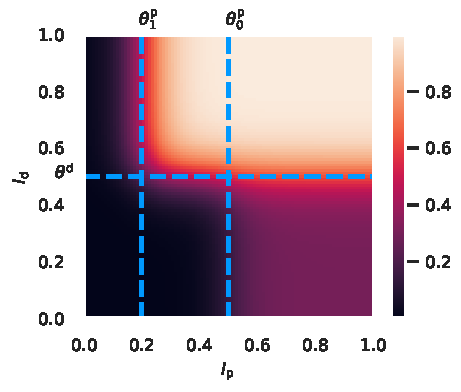
\includegraphics[width=0.6\textwidth]{./figures/plot_comp_mod_marks.pdf}
\caption{Output firing rate as a function of proximal and distal input as given by \eqref{eq:simpl_prox_dist}}
\label{fig:simpl_prox_dist}
\end{figure}

We expected the nonlinearity of the neuronal output to be selective for correlated proximal and distal input, such that a Hebbian learning rule allows the neuron to be selective to synaptic input generating the most coherence between distal and proximal input. We tested this hypothesis with a single neuron using the setup illustrated in Fig. \ref{fig:single_neuron_illustration}. The neuron receives $n=10$ proximal input signals $(y^{\rm p}_1(t),...y^{\rm p}_n(t)$ and a single distal input signal $y^{\rm d}(t)$. Proximal inputs were generated by simulating a chaotic random network and recording the activity of a randomly chosen unit. Each simulation run corresponds to a single proximal input signal to prevent possible correlations. The distal input was generated as a linear combination of the proximal input streams. In particular, we chose it to be an exact copy of $y^{\rm p}_1(t)$ as the most simple case for initial testing. Proximal weights were subject to Hebbian plasticity and weight normalization. The exact mathematical description of the setup is given in \eqref{eq:single_neur_0} -- \eqref{eq:single_neur_5} and Table \ref{tab:single_neuron_parameters}.

\begin{align}
I_{\rm p} (t) &= \sum_{k=1}^n w^{\rm p}_{k} (t) y^{\rm p}_{k} (t) \label{eq:single_neur_0} \\
y^{\rm d} (t) &= \sum_{k=1}^n a_k x^{\rm p}_{k} (t), \; \sum_{k=1}^n a_k = 1 \label{eq:single_neur_1} \\
I_{\rm d} (t) &= w^{\rm d} x^{\rm d} (t) \label{eq:single_neur_2} \\
y(t) &= \sigma\left(I_p(t)-\theta^{\rm p}_{1}\right) \sigma\left(I_d(t)-\theta^{\rm d}\right)\ +\alpha\sigma\left(I_p(t)-\theta^{\rm p}_{0}\right)\left[ 1 - \sigma\left(I_d(t)-\theta^{\rm d}\right)\right] \label{eq:single_neur_3} \\
\Delta w^{\rm p}_{i} (t) &= \epsilon_w  \left(y(t)-\langle y \rangle\right)\left(y^{\rm p}_{i}(t)-\langle y^{\rm p}_{i} \rangle \right) \label{eq:single_neur_4} \\
w^{\rm p}_{i}(t+1) &= w^{\rm p}_{\rm total} \frac{w^{\rm p}_{i}(t) + \Delta w^{\rm p}_{i}(t)}{\sum_{k=1}^n w^{\rm p}_{k}(t) + \Delta w^{\rm p}_{k}(t)} \label{eq:single_neur_5}
\end{align}

\begin{table}
\centering
\caption{Parameter settings for the setup described in \eqref{eq:single_neur_0} -- \eqref{eq:single_neur_5}.}
\begin{tabular}{|c|c|}
\hline
$w^{\rm d}$ & $1$ \\
$\theta^{\rm p}_{0}$ & $0.5$ \\
$\theta^{\rm p}_{1}$ & $0.2$ \\
$\theta^{\rm d}$ & $0.5$ \\
$\alpha$ & $0.3$ \\
$g$ & $5$ \\
$\epsilon_w$ & $10^{-3}$ \\
$w^{\rm p}_{\rm total}$ & $1$ \\
\hline
\end{tabular}
\label{tab:single_neuron_parameters}
\end{table}

\begin{figure}
\centering
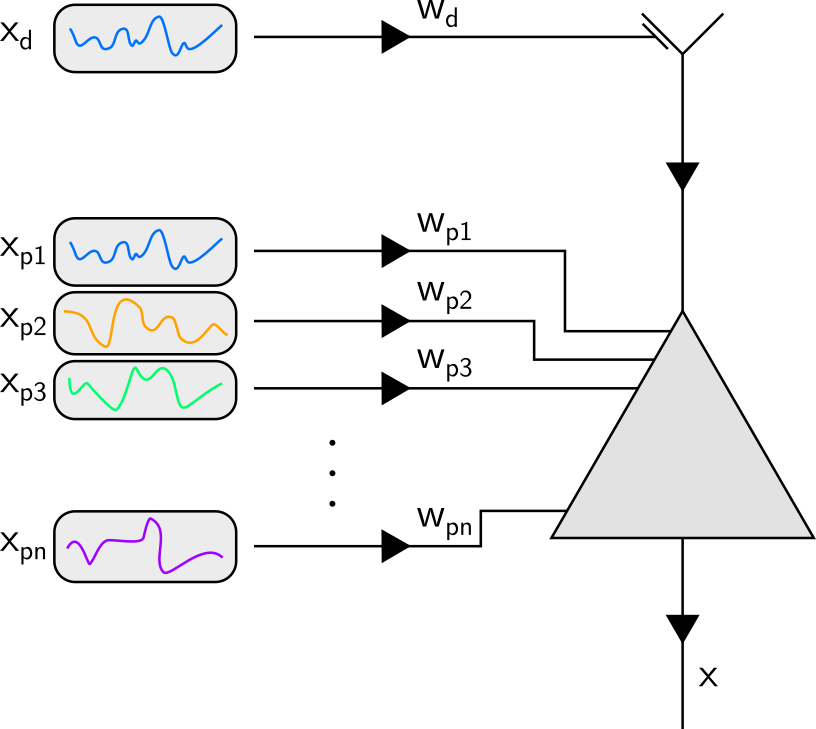
\includegraphics[width=6.91cm]{./figures/single_neuron_illustration.png}
\caption{A single neuron receiving multiple proximal inputs and a single distal signal.}
\label{fig:single_neuron_illustration}
\end{figure}

A First result is shown in Fig. \ref{fig:single_neuron_results_1}. The correct proximal weight is chosen such that the proximal total input follows the distal input signal. However, when testing the same setup except for a point-neuron summation of both proximal and distal inputs, the same result could be achieved, as shown in Fig. \ref{fig:single_neuron_results_2}. 

\begin{figure}
\centering
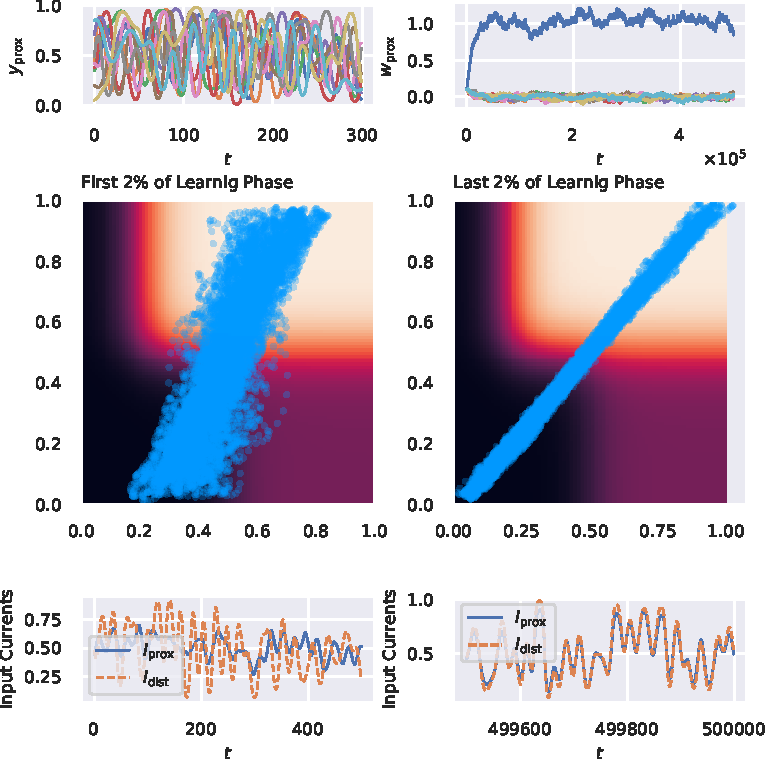
\includegraphics[width=\textwidth]{./figures/fig1.pdf}
\caption{Weights and input signals before and after Hebbian learning of proximal weights, using nonlinear proximal-distal interaction.}
\label{fig:single_neuron_results_1}
\end{figure}

\begin{figure}
\centering
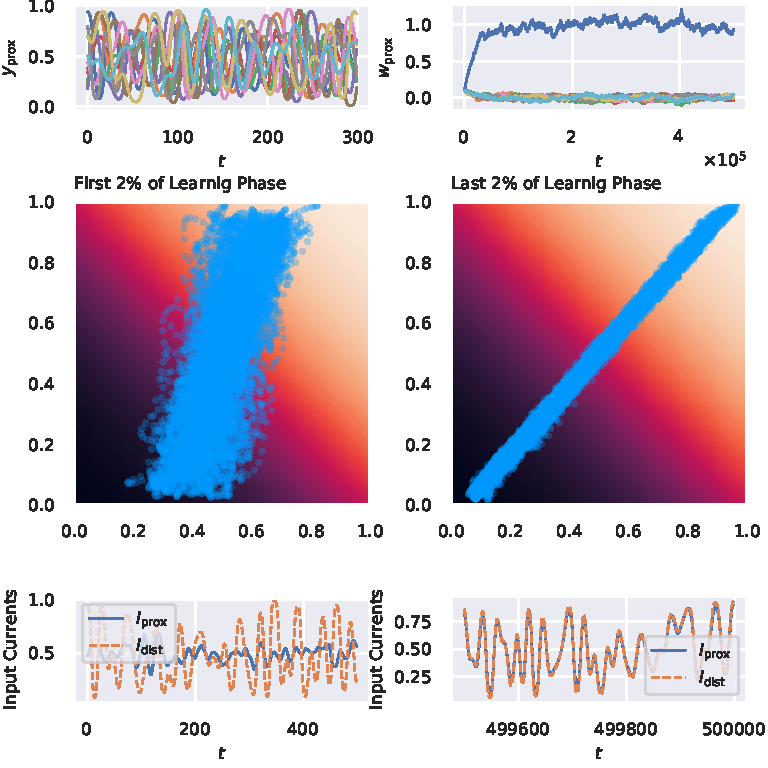
\includegraphics[width=\textwidth]{./figures/fig2.pdf}
\caption{Weights and input signals before and after Hebbian learning of proximal weights, using linear proximal-distal summation.}
\label{fig:single_neuron_results_2}
\end{figure}

As a further test, we doubled the standard deviation of the second proximal input, thereby making it preferential for the classic scheme of Hebbian learning combined with linear superposition of inputs. This revealed a difference between the proximal-distal activation function and the point neuron: While the proximal-distal scheme was able to select the proximal input that would maximize correlation between proximal and distal signals, the point neuron selected the principal component of the proximal input, in this case being the second input signal. These results are shown in Fig. \ref{fig:single_neuron_results_3} and \ref{fig:single_neuron_results_4}.

\begin{figure}
\centering
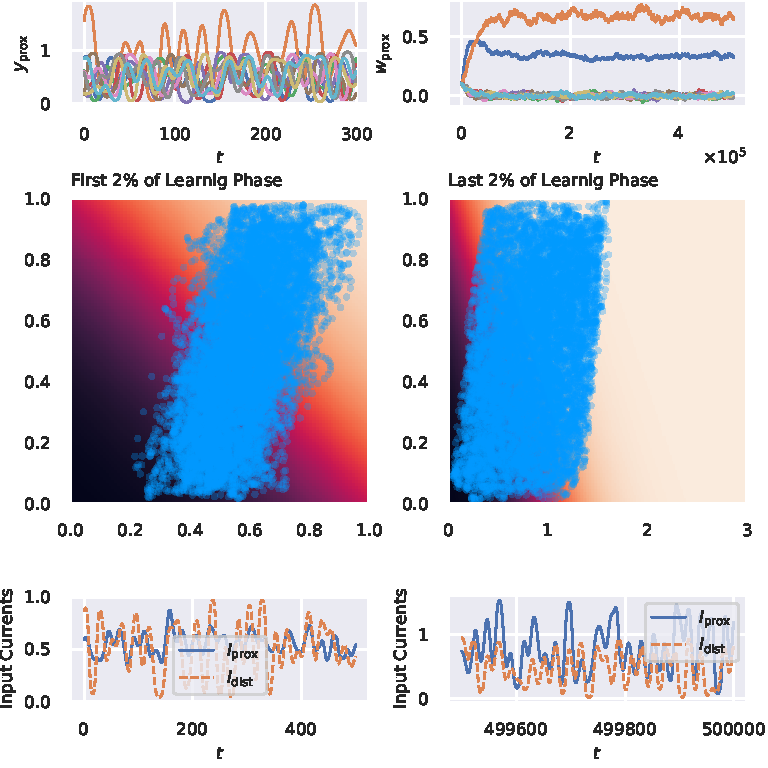
\includegraphics[width=\textwidth]{./figures/fig3.pdf}
\caption{Same setup as in Fig. \ref{fig:single_neuron_results_2}, but with the signal of the second proximal input channel scaled by a factor of two.}
\label{fig:single_neuron_results_3}
\end{figure}

\begin{figure}
\centering
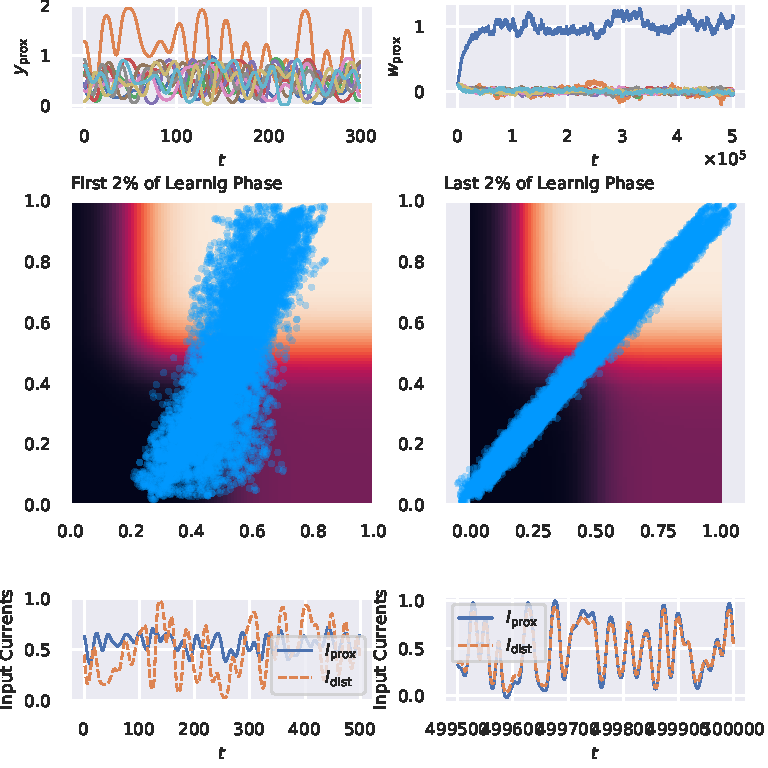
\includegraphics[width=\textwidth]{./figures/fig4.pdf}
\caption{Same setup as in Fig. \ref{fig:single_neuron_results_1}, but with the signal of the second proximal input channel scaled by a factor of two.}
\label{fig:single_neuron_results_4}
\end{figure}

\subsection{Output Dynamics After Learning}
In the given case that after learning, the proximal input as aligned to the distal input, one might consider the case where this alignment is temporarily broken. Which input conveys more information about the output? Of course, different scenarios might be considered here. First, we could consider the case where no input, or a constant level of input arrives at the distal compartment. This case is shown in Fig.~\ref{fig:const_dist_sweep_mod}. Changes in the distal input has a modulatory effect on the maximal output, but also shifts the bias. Speaking in terms of information transmission, this relates to two different effects: While changing the maximal output alters the overall impact of this neuron's efferent connections, changing the bias changes the actual gating for proximal input. 
%%%%%%%%%%%%%%%%%%%%
\begin{figure}
	\centering
	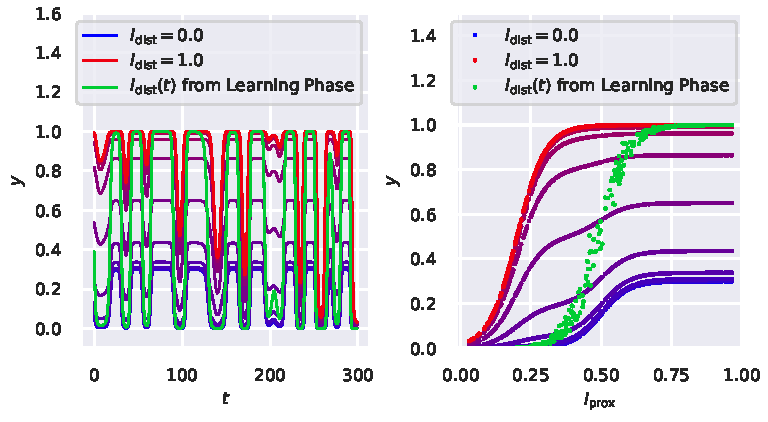
\includegraphics[width=\textwidth]{./figures/output_modulation_sweep.pdf}
	\caption{Output activity for a set of constant distal inputs (red to blue) applied after learning. Green line corresponds to the distal input also used for the learning phase.}
	\label{fig:const_dist_sweep_mod}
\end{figure}
%%%%%%%%%%%%%%%%%%%%
In the next scenario, we presented uncorrelated, fluctuating input to the distal compartment. In this case, we gradually increased the maximum value for the distal input from zero to one, see Fig.~\ref{fig:altern_dist_sweep_mod}. Obviously, increased fluctuations in $I_{\rm d}$ made it harder to actually extract information about $I_{\rm p}$ from the output. Therefore, one might wonder which input stream conveys more information to the output activity, given that both are uncorrelated and have the same overall strength. This is illustrated in Fig.~\ref{fig:output_mod_project}. Although the projection onto the distal input space resulted in a wider spread of activity for strong driving, a numerical estimate of the mutual information resulted in $I(I_{\rm d};y) \approx 2.75$ bits and $I(I_{\rm p};y) \approx 1.87$ bits, respectively. This indicates that in the described scenario, the distal input actually conveys more information about the output as compared to the proximal input.

%%%%%%%%%%%%%%%%%%%%
\begin{figure}
	\centering
	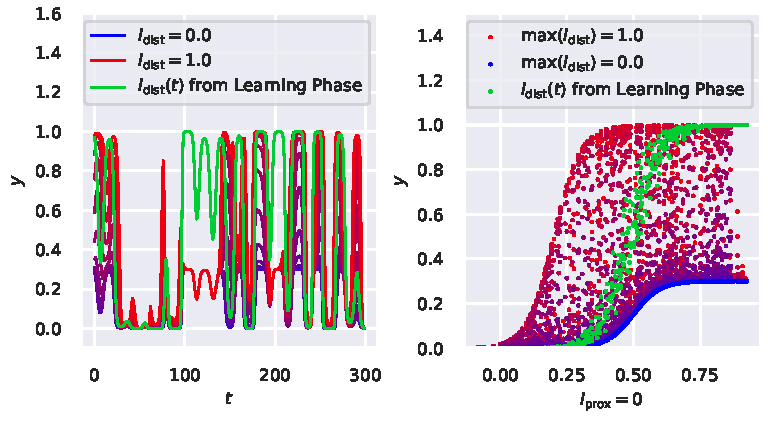
\includegraphics[width=\textwidth]{./figures/output_modulation_sweep_decorr_input.pdf}
	\caption{Output activity for a set of fluctuating distal inputs (red to blue) that are uncorrelated with the proximal input (applied after learning). Green line corresponds to the distal input also used for the learning phase.}
	\label{fig:altern_dist_sweep_mod}
\end{figure}
%%%%%%%%%%%%%%%%%%%%

%%%%%%%%%%%%%%%%%%%
\begin{figure}
	\centering
	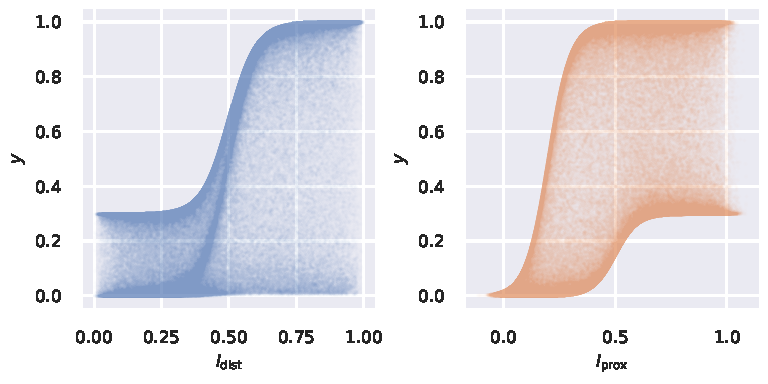
\includegraphics[width=\textwidth]{./figures/output_modulation_max_distal.pdf}
	\caption{Activity for independently fluctuating values of $I_{\rm d}$ and $I_{\rm p}$ both ranging from $0$ to $1$, projected onto $I_{\rm d}$ (left) and $I_{\rm p}$ (right).}
	\label{fig:output_mod_project}
\end{figure}
%%%%%%%%%%%%%%%%%%%

\subsection{Analytic Approximation of Weight Dynamics}

Assuming that inputs to \eqref{eq:simpl_prox_dist} practically never reach a region where $\theta_{p1}$ becomes relevant, we remove this threshold, resulting in:
\begin{equation}
x\left(I_p,I_d\right) = \sigma\left(I_d-\theta_d\right)\ + \alpha\sigma\left(I_p-\theta_{p0}\right)\sigma\left(-\left(I_d-\theta_d\right)\right) \; . \label{eq:simpl_further_prox_dist}
\end{equation}
We can set both thresholds to zero without loss of generality by assuming that $\langle I_p \rangle = 0$ and $\langle I_d \rangle = 0$.

To approximate the weight dynamics, we expand the activation function around the mean input (being zero by assumption) to first order. This gives
\begin{equation}
y\left(I_{\rm p},I_{\rm d}\right) =  y_0 + p \cdot g \alpha/2  + d \cdot g \left(1-\alpha/2\right) + \mathcal{O}(I_{\rm p}^2,I_{\rm d}^2) \; .
\end{equation}
Plugging this approximation into \eqref{eq:single_neur_4}, we get
\begin{equation}
\Delta w^{\rm p}_{i} \approx \epsilon_w g \left( I_{\rm p} \alpha/2  + I_{\rm d}(1-\alpha/2) -\langle  I_{\rm p} \alpha/2  + I_{\rm p}(1-\alpha/2) \rangle\right)\left(x^{\rm p}_{i}(t)-\langle x^{\rm p}_{i} \rangle \right)
\end{equation}
Further simplification of this equation leads to
\begin{align}
\Delta w^{\rm p}_{i} &\approx \epsilon'_w \left[\alpha \sum_j  C^{yy}_{ij} w^{\rm p}_{j} + (2-\alpha) C^{dy}_i \label{eq:approx_delta_w}\right] \\
\epsilon'_w &\equiv \epsilon_w g /2 \\
C^{yy}_{ij} &\equiv \avg{\left(y^{\rm p}_{i} - \avg{y^{\rm p}_{i}} \right)\left( y^{\rm p}_{j} - \avg{y^{\rm p}_{j}} \right)} \\
C^{dy}_i &\equiv \avg{\left(d - \avg{d} \right) \left(y^{\rm p}_{i} - \avg{y^{\rm p}_{i}} \right)}
\end{align}

%For a first comparison between full weight dynamics and approximation, see Fig. \ref{fig:weight_dyn_analytic_comp} (!!Better plot to come!!).

%\begin{figure}
%\centering
%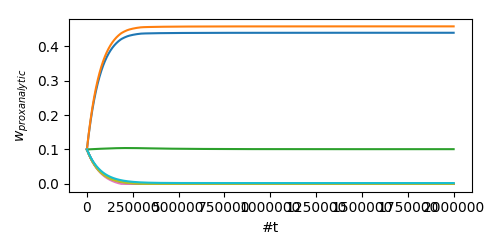
\includegraphics[width=0.8\textwidth]{./figures/weights_analytic_comp.png}
%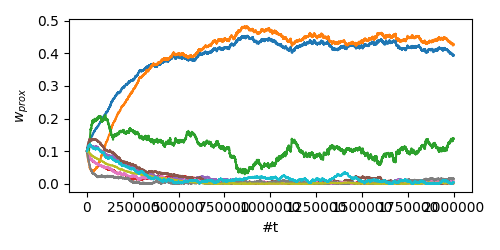
\includegraphics[width=0.8\textwidth]{./figures/weights_full_sim_comp.png}
%\caption{Comparison of weight dynamics between analytic approximation and full simulation.}
%\label{fig:weight_dyn_analytic_comp}
%\end{figure}

We can compare \eqref{eq:approx_delta_w} with the expression that we get if we calculate the negative derivative of the mean squared error between proximal and distal input, scaled by some arbitrary proportionality factor $\gamma$:
\begin{equation}
\Delta w^{\rm p}_{i} \propto -\partial_{w^{\rm p}_{i}} \frac{1}{2}\avg{\left( I_{\rm p} -\gamma I_{\rm d} \right)^2} = -\sum_j C^{yy}_{ij} w^{\rm p}_{j} + \gamma C^{dy}_i \; . \label{eq:mse_diff}
\end{equation} 
Note that if we set $\alpha$ to negative values, this equation would have the same mathematical form as \eqref{eq:approx_delta_w}.

What has not been included in this analysis yet is synaptic normalization. In this respect, it is important to note that the fixed point that one would get from $\Delta w^{\rm p}_{i} = 0, \; \forall i$ is not the fixed point that is actually attained during the learning process since it is generally not compatible with the normalization condition $\left\lVert \mathbf{w} \right\rVert_1 = 1$. Rather, stable weights are achieved by a positive feedback on the weights which is constantly canceled by the synaptic normalization. By defining
\begin{align}
	\widehat{A} &\equiv \alpha \widehat{C}^{yy} \\
	\mathbf{b} &\equiv (2-\alpha) \mathbf{C}^{dy}
\end{align}
and omitting the p-superscript in the proximal weights, the actual stationarity condition is given by
\begin{equation}
	\frac{\left(1 + \epsilon'_w \widehat{A}\right)\mathbf{w} + \epsilon'_w \mathbf{b}}{\left\lVert \left(1 + \epsilon'_w \widehat{A}\right)\mathbf{w} + \epsilon'_w \mathbf{b} \right\rVert_1} = \mathbf{w} \label{eq:stab_cond_w}
\end{equation}
where $\left\lVert \cdot \right\rVert_1$ denotes the $\ell_1$ norm.

Expanding this expression to first order gives
\begin{align}
	\mathbf{w} + \epsilon'_w \left[\frac{\widehat{A}\mathbf{w} + \mathbf{b}}{\left\lVert \mathbf{w} \right\rVert_1} - \frac{\mathbf{w}}{\left\lVert \mathbf{w} \right\rVert_1^2}\left\lVert \widehat{A}\mathbf{w} + \mathbf{b}\right\rVert_1\right] &= \mathbf{w} \\
	\widehat{A}\mathbf{w} + \mathbf{b} - \mathbf{w}\left\lVert \widehat{A}\mathbf{w} + \mathbf{b}\right\rVert_1 &= 0 \; ,
\end{align}
using the fact that $\left\lVert \mathbf{w} \right\rVert_1 = 1$ by construction. In the special case of $\widehat{A}$ being simply a rescaled identity matrix, the solution would be $\mathbf{w} = \mathbf{b} / \left\lVert \mathbf{b} \right\rVert_1$. Moreover, the fixpoint of \eqref{eq:mse_diff} would also be aligned with $\mathbf{w} = \mathbf{b}$. An alternative case where $\mathbf{b} / \left\lVert \mathbf{b} \right\rVert_1$ would be an approximately correct solution of \eqref{eq:stab_cond_w} is when $\widehat{C}^{yy}$ is weak compared to $\mathbf{C}^{dy}$. However, decreasing the overall scale $\widehat{C}^{yy}$ does not affect the direction of $\mathbf{w}$ corresponding to the fixpoint of \eqref{eq:mse_diff}. Therefore, differences in the alignment between the solutions of \eqref{eq:mse_diff} and \eqref{eq:stab_cond_w} are to be expected.

It should be noted that $\mathbf{w} = \mathbf{b} / \left\lVert \mathbf{b} \right\rVert_1$ is also the stationary solution of a learning rule trying to maximize the covariance between $I_{\rm p}$ and $I_{\rm d}$ under a multiplicative normalization constraint, since (omitting means)
\begin{equation}
	\partial_{\mathbf{w}^{\rm p}} \left\langle I_{\rm p}I_{\rm d}\right\rangle = \left\langle \mathbf{y} I_{\rm d} \right\rangle = \mathbf{C}^{dy} \; .
\end{equation}
However, maximizing covariance is not necessarily the same as maximizing correlation:
\begin{equation}
	\partial_{\mathbf{w}^{\rm p}} \rho\left(I_{\rm p},I_{\rm p}\right) \propto \mathbf{C}^{dy} - \left[{\mathbf{w}^{\rm p}}^T \widehat{C}^{yy}{\mathbf{w}^{\rm p}}\right]\left[{\mathbf{w}^{\rm p}}^T \mathbf{C}^{dy} \right] \widehat{C}^{yy}{\mathbf{w}^{\rm p}}
\end{equation} .
%\subsection{Adding Plasticity to the Distal Input}
%\label{sect:dist_plast}
%
%Instead of a single fixed distal input, we used multiple distal inputs with weights $w_{\rm dist, i}$ and applied the same plasticity rule as in \eqref{eq:single_neur_4} and \eqref{eq:single_neur_5}. The input currents were drawn from the same chaotic sequences, where the principle component was aligned with the first input stream, as shown in Fig.~\ref{fig:dist_plast_comp}B (blue trace). The plasticity rule selected this PC from the distal input (Fig.~\ref{fig:dist_plast_comp}C), which allowed the proximal input weights to also align with this component, even though we set the PC of the proximal input to be aligned with the second input stream as a ``distraction", see Fig.~\ref{fig:dist_plast_comp}B,C.
%
%\begin{figure}
%\centering
%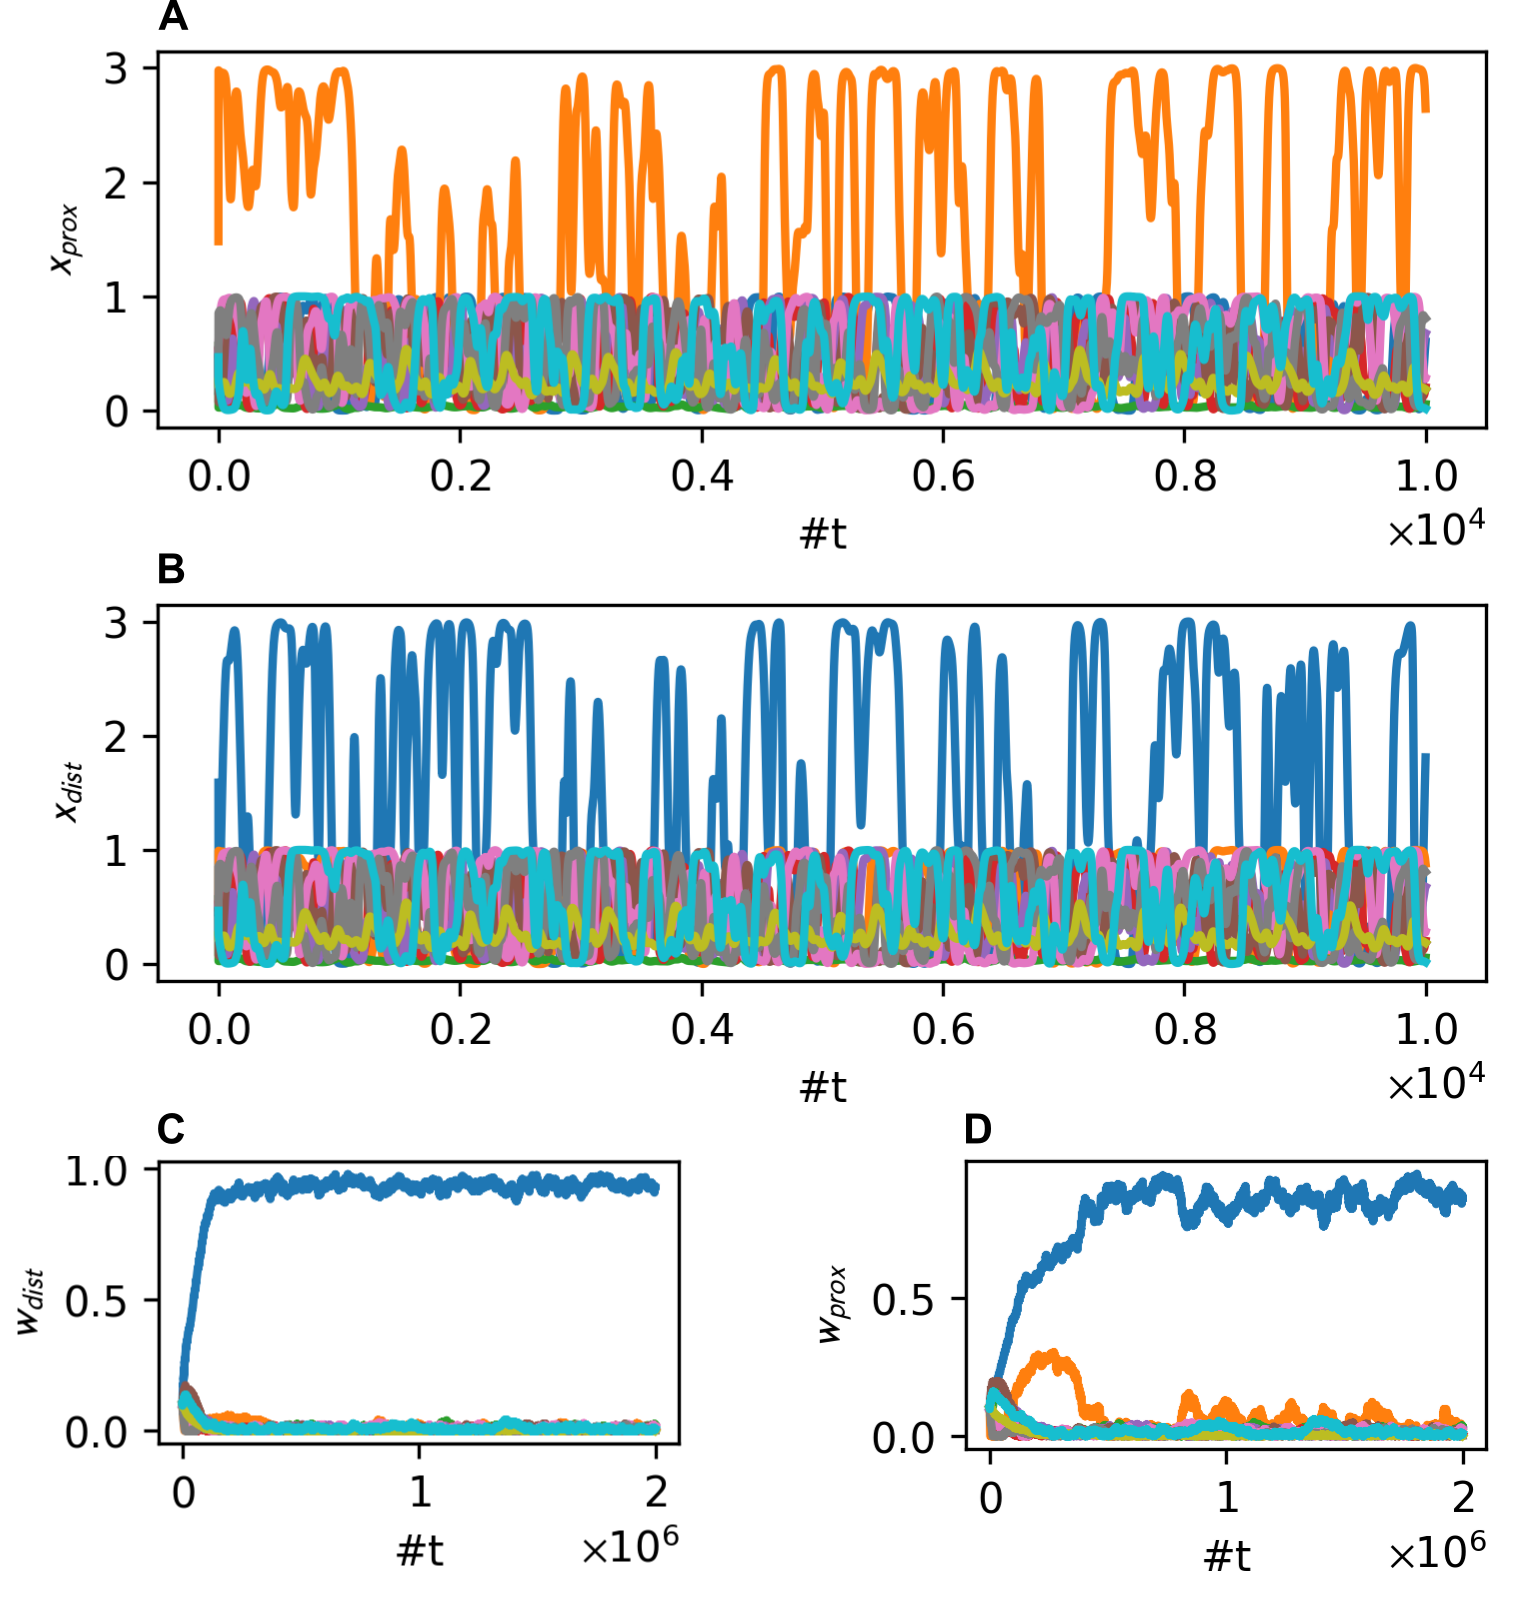
\includegraphics[width=\textwidth]{./figures/dist_plast_comp.png}
%\caption{Proximal and distal inputs generated by chaotic sequences ({\bf A},{\bf B}) and the corresponding weight dynamics ({\bf C},{\bf D})}
%\label{fig:dist_plast_comp}
%\end{figure}
%
%%\subsubsection{$\rm Ca^{2+}$ Spikes Explain Two Separate Modes of Output Activity}
%%A study on a two-compartment model of coupled two-dimensional spiking neuron models has shown that the generation of $\rm Ca^{2+}$ in the dendritic compartment provides an explanation for the appearance of a sharp transition between fast-firing and slow-firing somatic activity \cite{Yi_2017}.
%
%
%
%\subsection{Application to a Recurrent Network}
%
%Using the previously described mechanism, we would like to predict an input sequence in a network architecture depicted in Fig. \ref{fig:prox_dist_recurrent}. More precisely, we want the proximal input arriving at the node(s) that were separated in the illustration to be a prediction of the distal input arriving at the same node(s).
%\begin{figure}
%\centering
%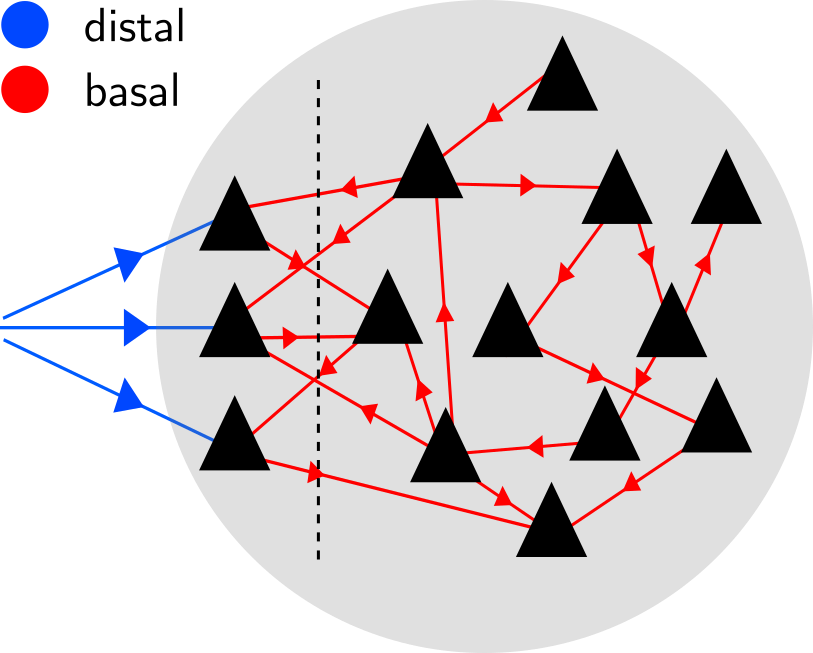
\includegraphics[width=0.5\textwidth]{./figures/prox_dist_rnn_illustration.png}
%\caption{Combining correlation-sensitive learning with a recurrent reservoir.}
%\label{fig:prox_dist_recurrent}
%\end{figure}
%
%
%\subsubsection{Test with a Gradient Descent Rule}
%One problem of this setup is the fact that the not yet correlated proximal input to the nodes collecting the proximal input might impede a proper encoding of the distal input signal in the recurrent reservoir. Therefore, we ran a test with the following setup: A single ``hub" node with a proximal-distal activation function was connected to a recurrent reservoir of $N=300$ nodes. The reservoir itself consisted of simple $\rm tanh$ point neurons and a sparse ($p=0.1$) random Gaussian connectivity matrix, drawn from $\mathcal{N}(\mu=0,\sigma=g/\sqrt{pN})$. The connections from the ``hub" node into the recurrent reservoir were fully connected and drawn from $\mathcal{N}(\mu=0,\sigma=1)$. Settings for the proximal-distal activation function as well as for the distal weight were set to the same values as in the previous section. For this test, we used a gradient descent rule for the learning of the proximal weights coming from the reservoir nodes $x_i$, reading
%\begin{equation}
%\Delta w_i(t) = \epsilon_w \left(I_p(t)-I_d(t)\right) x_i \;.
%\end{equation}
%The results are shown in Fig. \ref{fig:echo_state_network_pd_act_grad_desc}.
%
%\begin{figure}
%\centering
%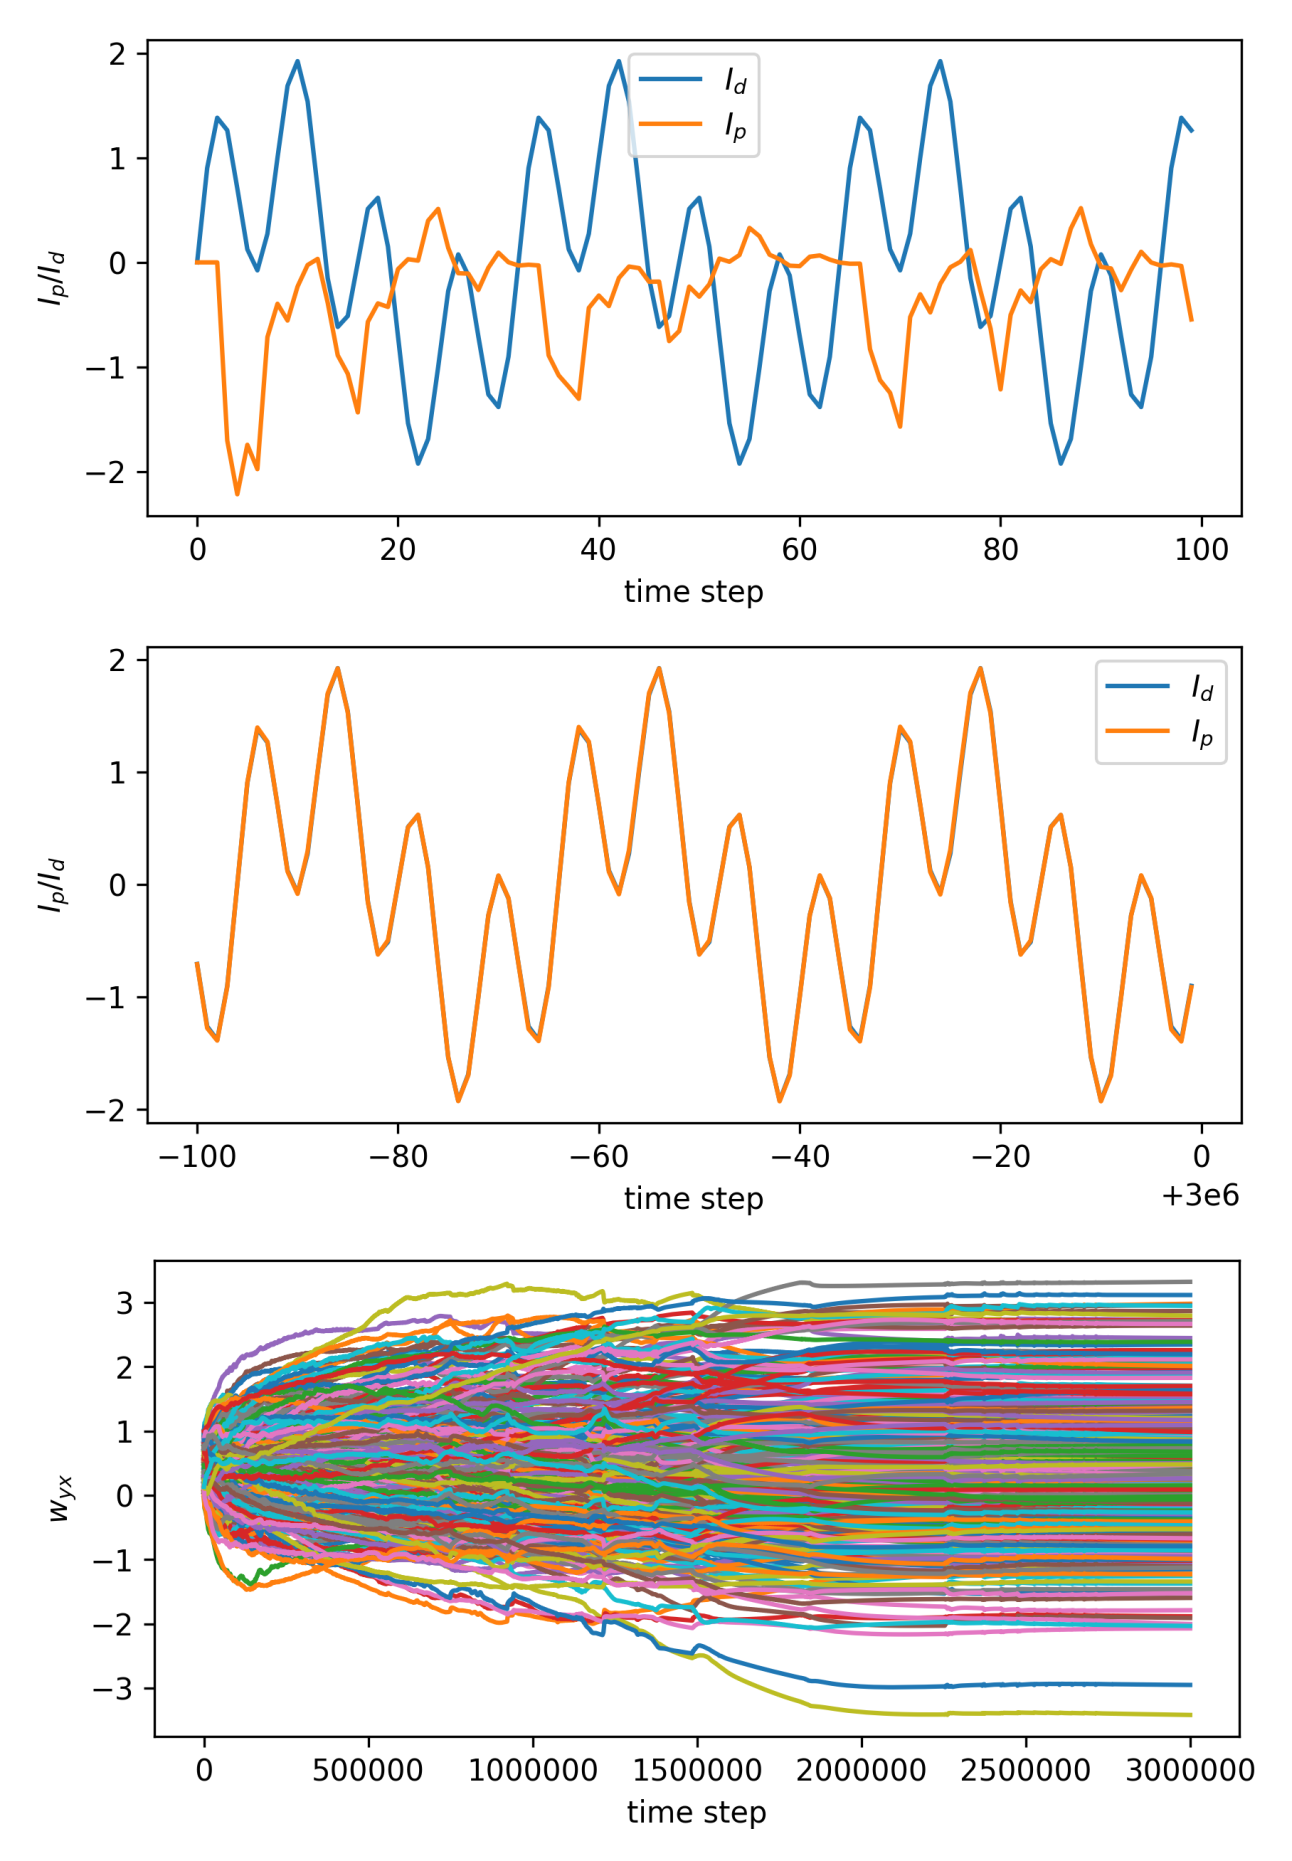
\includegraphics[width=\textwidth]{./figures/echo_state_network_pd_act_grad_desc.png}
%\caption{Proximal and distal signal before and after learning, proximal weights during learning}
%\label{fig:echo_state_network_pd_act_grad_desc}
%\end{figure}
%
%%
%%...Still to be done:
%%\begin{itemize}
%%\item Hebbian learning rule instead of gradient descent?
%%\item Use p.-d. activation in the reservoir. Problem: Requires more tuning of parameters (thresholds etc.) to get the ``echo-state property".
%%\item Is this a good architecture for generalization/multiple layers? Where do feed forward connections go in?
%%\end{itemize}

\subsection{Effect of ``Distraction" Components in the Proximal Input}
As already seen previously, using a compartment model forces proximal inputs to a configuration that aligns with the presented distal input, even if the proximal input has a direction of larger variance that does not align with the weight configuration that matches the distal input. We wanted to further quantify this effect systematically. To do so, we devised the following setup: A random sequence for the distal input was generated using the construction given by \eqref{eq:single_neur_1}, that is, a random linear combination of the sequences also presented to the proximal input. However, the proximal input was also subject to a distracting scaling operation perpendicular to the vector $\mathbf{a}$ that defined the linear combination for the distal input. Since the number of proximal input $N_p = 10$ was larger than $2$, this was done by picking a random unit vector in the hyperplane that is orthogonal to $\mathbf{a}$ and then stretching the $N_p$-dimensional input by a factor $s$ along this direction. Therefore, this procedure simulated a ``worst-case scenario" where the proximal input has its greatest variance in a direction perfectly orthogonal to the desired alignment of the weights. For a given scaling factor $s$, we generated multiple trials of this simulation and then calculated the resulting normalized mean squared error
\begin{equation}
	MSE = \frac{\left\langle \left\lvert \mathbf{a} - \mathbf{w}^{\rm p} \right\rvert^2\right\rangle}{\left\langle \left\lvert \mathbf{a}\right\rvert^2\right\rangle} \; .
\end{equation}
This was done over a range of values of $s$. The results are shown in Fig.~\ref{fig:distraction_scaling}. The compartment model preserves a much better alignment for larger values of $s$, with practically zero error up to a factor of approximately $2.5$.

An alternative protocol was used in Fig.~\ref{fig:distraction_inputs}: Here, $N_p = 20$ and the distal input was composed of the average of $10$ randomly picked sequences. As a distraction for the proximal input, $N$ proximal inputs \emph{other} than those chosen to construct the distal input were elevated by a factor of $2$. Apart from the fact that, like in the previous protocol, the point neuron falls short in aligning the proximal weights, it is interesting to note that increasing the number of distracting inputs decreased its mean squared error. Presumably, this is can be explained by noting that an increased number of elevated inputs makes for a less clearly pronounced first principal component as compared to all other components.



\begin{figure}
	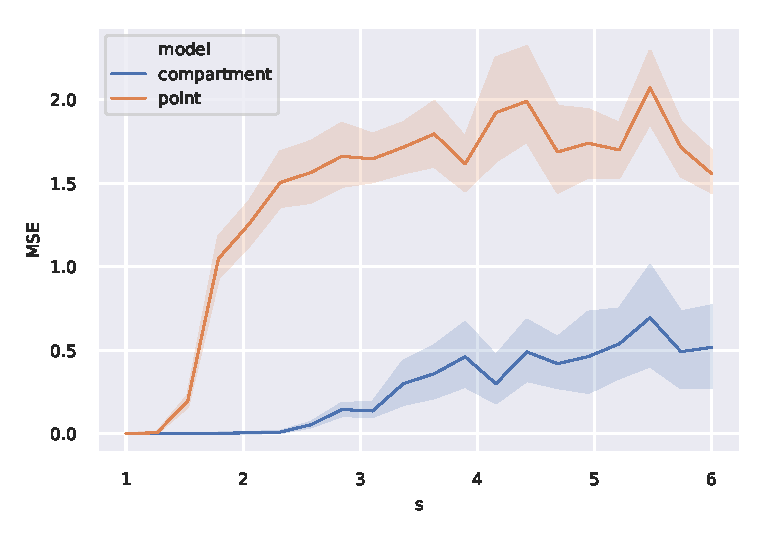
\includegraphics[width=\textwidth]{./figures/distraction_scaling.pdf}
	\caption{Normalized mean squared error between $\mathbf{w}^{\rm p}$ and vector $\mathbf{a}$ defining the linear combination of signals presented to the distal input for a given distraction scaling $s$.}
	\label{fig:distraction_scaling}
\end{figure}

\begin{figure}
	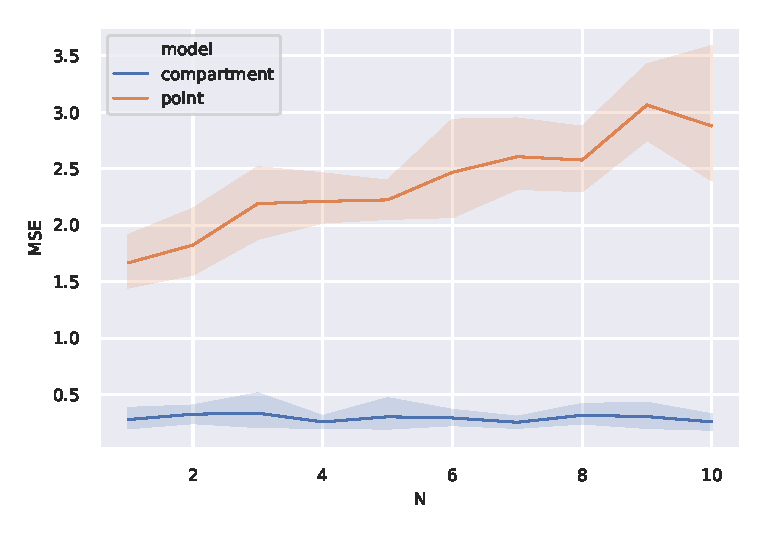
\includegraphics[width=\textwidth]{./figures/distraction_inputs.pdf}
	\caption{Normalized mean squared error between $\mathbf{w}^{\rm p}$ and vector $\mathbf{a}$ as a function of the number of proximal inputs being elevated in signal strength as a distraction.}
	\label{fig:distraction_inputs}
\end{figure}

\subsection{Pattern Classification Task}

We wanted to test the ability of our compartment model to learn to binary classify proximal input patterns. During the learning phase, activity patterns of dimension $500$ were presented to the proximal input while a single distal input encoded the binary classification of these patterns. Before actually simulating the learning, $P$ patterns were generated by randomly setting $10\%$ of the proximal inputs to $1$, leaving the rest at $0$. We randomly assigned each of those patterns to either of the two classes with equal chance (after checking that all random patterns were unique). The actual training sequence was then generated by repeatedly drawing samples from this predefined set of patterns and presenting them to the proximal input, as well as the feeding the respective $0/1$ activity encoding the binary classification into to the distal input. We tested this procedure both with the compartment model as well as a simple point neuron where $y(I_{\rm p},I_{\rm d}) = \sigma(I_{\rm p}+I_{\rm d} - \theta)$, with $\theta = 1$. Furthermore, we gradually increased the size of the set of patterns $P$. To test the actual classification performance, another random sequence from the pattern set was generated, however, this time switching off the distal input. A pattern was then classified as class $1$ if the activity exceeded $\alpha/2$, that is, half of the maximally achievable activity in the absence of distal input. The resulting accuracy shown in Fig.~\ref{fig:class_accuracy} was estimated by the fraction of correctly classified input patterns. Apparently, a point neuron can achieve similar accuracy levels under the given experimental setup. It should be noted though that both models fall short to a perceptron model with a simple perceptron learning rule, which essentially represents the upper accuracy limit for this linear classification task. One reason why the two other models performed worse could be due to the enforced positivity of the weights, which was done for reasons of biological plausibility. Removing this constraint indeed resulted in better performance in the compartment and point model, as as shown in Fig.~\ref{fig:class_accuracy_no_constraint}. However, substantial differences between these two models could still not be observed.

\begin{figure}
	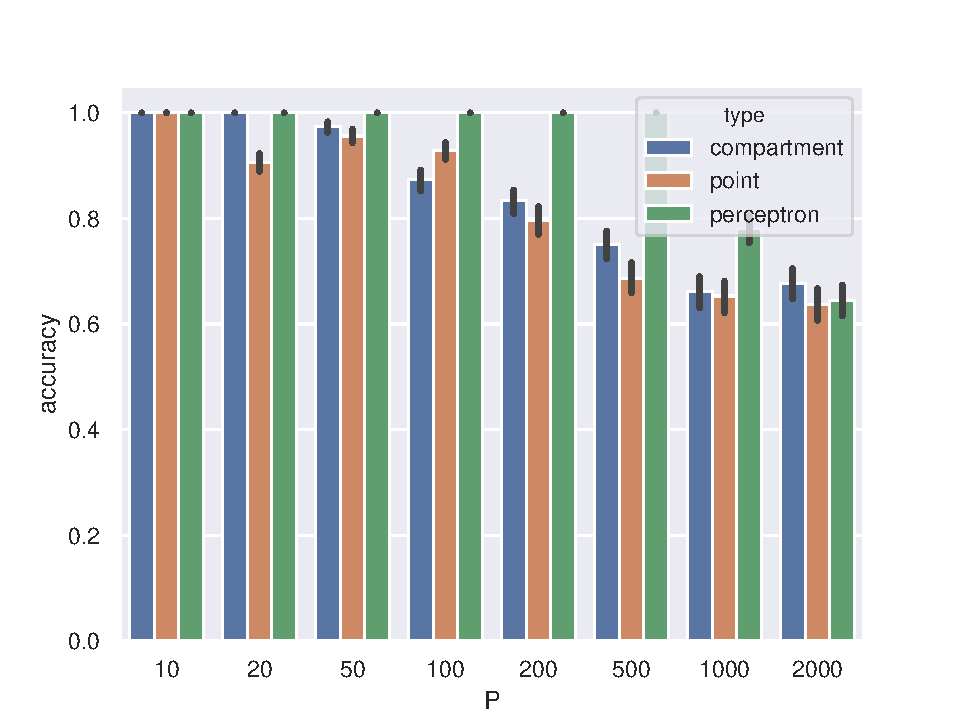
\includegraphics[width=\textwidth]{./figures/accuracy_pattern_number.pdf}
	\caption{Binary classification accuracy for different amounts of training patterns and different neuron models.}
	\label{fig:class_accuracy}
\end{figure}

\begin{figure}
	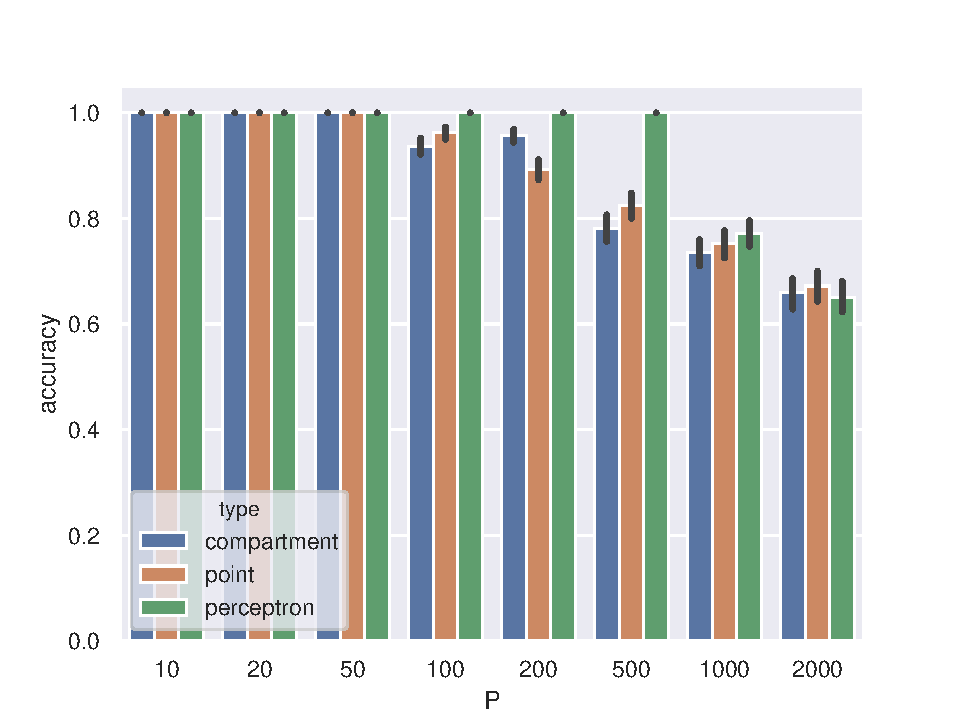
\includegraphics[width=\textwidth]{./figures/accuracy_pattern_number_no_constraint.pdf}
	\caption{Binary classification accuracy for different amounts of training patterns and different neuron models. Same setup as in Fig.~\ref{fig:class_accuracy}, but allowing for negative weights in the point and compartment model}
	\label{fig:class_accuracy_no_constraint}
\end{figure}

Another issue not yet addressed is the fact that biases were adjusted to fit the average appearance of the two classes, that is, with equal probabilities. If we change this so that e.g. class $0$ has a $90\%$ chance of being present, we should expect lower performance under the same set of parameters. This case actually corresponds to a more realistic scenario where cells are sensitive to a more specific set of patterns, thus being activated more sparsely. The results are shown in Fig.~\ref{fig:class_accuracy_imbalance}. As expected, Hebbian learning of the weights can not account for this imbalance, whereas perceptron learning is unaffected. Of course, one could easily fix this by simply introducing some homeostatic mechanisms that adjusts the average activity to fit a given prior probability of finding the patterns that the neuron is supposed to react to. However, this is a ad-hoc solution rather than a biological explanation, except if we argue that there is ac certain heterogeneity among average neural activities and that eventually, neurons will develop receptive fields for patterns whose prior probabilities fit the neurons' given average activity.

\begin{figure}
	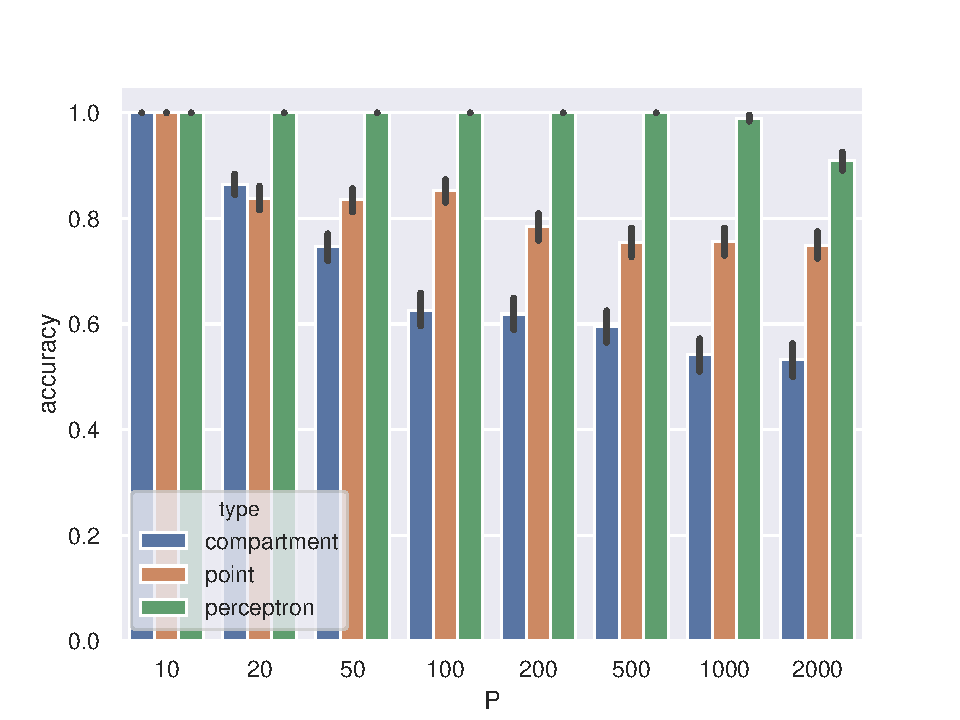
\includegraphics[width=\textwidth]{./figures/accuracy_pattern_number_class_imbalance.pdf}
	\caption{Binary classification accuracy for different amounts of training patterns and different neuron models. Same setup as in Fig.~\ref{fig:class_accuracy}, but with class $0$ appearing with $90\%$ probability (as opposed to a $50/50$ chance as in the previous setups).}
	\label{fig:class_accuracy_imbalance}
\end{figure}

Similar to what was investigated in Fig.~\ref{fig:distraction_inputs}, we also tested the classification accuracy against distraction patterns with different amounts of active nodes that were orthogonal to the actual ``learnable" activity patterns and scaled up by a factor of $2$. Prior probabilities of the binary classification were kept at $50\%$ in this case and the number of different classification and distraction patterns was both set to $100$. The proximal input used during learning was then generated by adding a randomly picked distraction pattern onto a random classification pattern in each iteration. The distal input still simply encoded the class associated with the respective classification pattern. Ideally, the neuron would learn to filter out the proximal information relevant for the classification, despite an increasing impact of the distraction patterns on the overall output activity. The results shown in Fig.~\ref{fig:distraction_patterns} were acquired by testing the performance after learning without the distraction patterns. Though not being very prominent, one can observe a slight advantage of the compartment model over the point neuron. This is consistent with our interpretation of the plasticity in the compartment model being mostly driven by coincidence detection between the proximal and distal input, while the proximal plasticity in the point neuron is more affected by the direction of largest variance in the proximal input space.

When testing the performance after learning with the distraction patterns being present, we found the same overall trend where the compartment model performed slightly better than the point neuron, see Fig.~\ref{fig:distraction_patterns_2}. Obviously, though, the accuracy decreased for all types of models and learning procedures.

\begin{figure}
	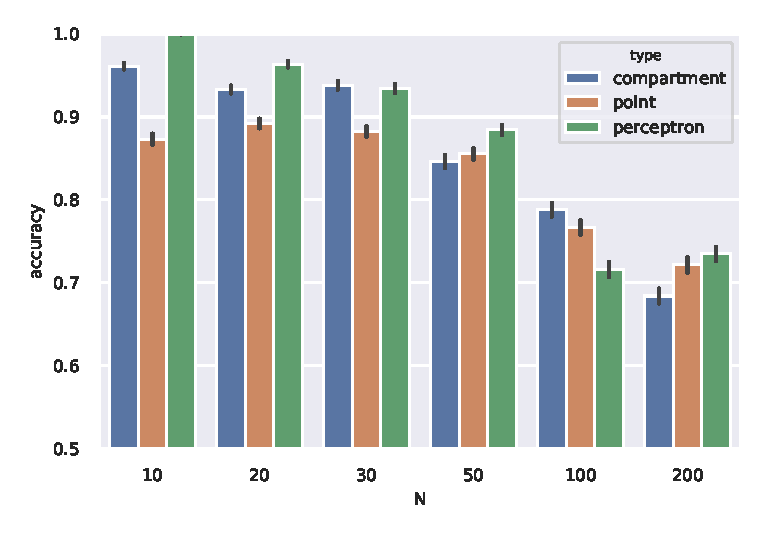
\includegraphics[width=\textwidth]{./figures/accuracy_distraction_patterns_no_distraction_during_testing.pdf}
	\caption{Classification accuracy for different neuron models and a different number of active nodes in the ``distraction patterns" during the learning phase. Distraction input was turned off during testing. Averaged over $10$ simulation runs.}
	\label{fig:distraction_patterns}
\end{figure}

\begin{figure}
	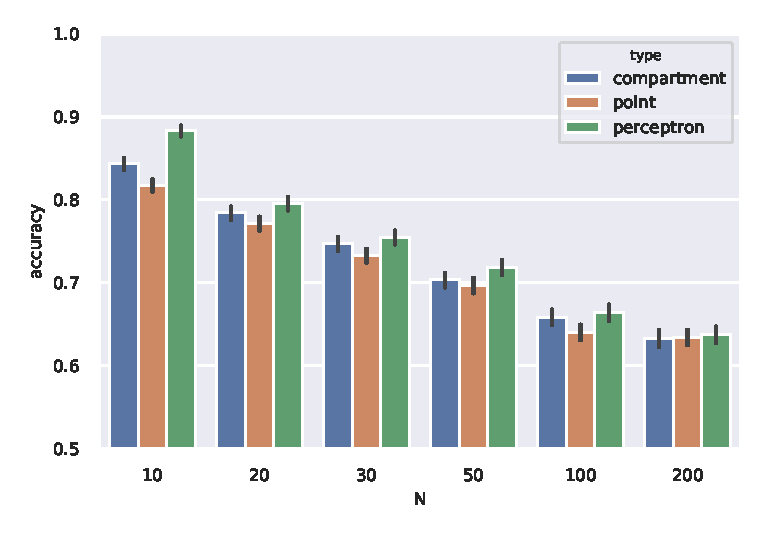
\includegraphics[width=\textwidth]{./figures/accuracy_distraction_patterns_distraction_during_testing.pdf}
	\caption{Classification accuracy for different neuron models and a different number of active nodes in the ``distraction patterns" during the learning phase. Distraction input was turned off during testing. Averaged over $10$ simulation runs.}
	\label{fig:distraction_patterns_2}
\end{figure}



%\subsection{Comparison to a Two-Compartment Model with Error Minimization}
%In a publication by Urbanczik and Senn, somatic and dendritic interaction takes place in a two-compartment approach, where both compartments are modeled as passive capacitors \cite{Urbanczik_2014}. Somatic spiking is modeled as a Poisson process with a rate given by the sigmoid function of the somatic voltage. In contrast to our model, dendritic plasticity is then driven by an error term between somatic spiking activity and the activity that would be present in the soma if only dendritic input was present. This allows single neurons to precisely learn a teaching signal. Furthermore, it was shown that such a learning algorithm allows the formation of associative memory in a recurrent network, as well as the emergence of feed-forward topographic maps (onto the dendritic compartment). The authors claim that using the two-compartment model justifies the use of an error driven plasticity rule. While it is reasonable that compartments could temporally store two different values---voltages in this case---which are to be compared, it is not obvious how such a comparison might be implemented. In particular, the rule proposed in the paper contains some hypothetical somatic activity, derived from the dendritic voltage, whose biological origin remains unclear.
%
%
%
%%\subsection{Interpretation of the Results}
%%
%%As a minimal interpretation of the observed effects, we denote that our activation function gives distal inputs a stronger influence on postsynaptic activity than somatic input. In fact, if both proximal and distal weights obey the same learning principle, the linearized plasticity rule \eqref{eq:approx_delta_w} reduces to a simple Hebbian covariance learning rule, where proximal inputs are pre-amplified by a factor $\alpha$ and distal inputs by a factor $2-\alpha$. As such, learning still convergences to the principle component of the rescaled inputs.
%%
%%Even though this reduction of the learning process to the linearized case might let the presented results appear ``trivial", the advantage of the full nonlinear activation function becomes apparent in the absence of distal inputs: non-zero postsynaptic activity can be achieved with much less somatic input than what one would expect in the linear/point neuron case.
%
%\subsection{Physiological Basis of the Architecture}
%\begin{itemize}
%	\item Feedback connections project from L5 to L1/2 \cite{Barbas_2015}. However, there is no evidence that feedback connections terminate \emph{exclusively} at the apical parts of L5 neurons \cite{Larkum_2018}. Therefore, the functioning or mode of operation of these feedback connections might change depending on their termination site.
%	\item In the predictive coding scheme, feedback connections are actually assumed to be mostly inhibitory \cite{Bastos_2012}. The common picture is that predictive feedback tries to eliminate or cancel out input from feed-forward or later connections. A possible explanatory mechanism could be via inhibitory interneurons \cite{Meyer_2011}.
%	\item Feed-forward connections project from L4/5 to L5 \cite{Barbas_2015}
%\end{itemize}
%
%\subsubsection{What is the Right Plasticity Rule for Distal Synapses?}
%While a simple Hebbian rule is a plausible candidate for proximal plasticity, experimental studies suggest that distal synapses can actually undergo LTP or LTD, depending on the mode of neural firing \cite{Sjoestroem_2006,Letzkus_2006}: So-called backpropagation-activated calcium spikes (BACs), which appear as bursts of action potentials, can be elicited when both basal and apical excitatory input is present. In this case, LTP (i.e. regular Hebbian-like) plasticity can be observed in the apical synapses. However, in the absence of this firing mode, apical synapses tend to undergo LTD, which could be described as a form of anti-Hebbian plasticity. Fig.~\ref{fig:ltp_switch} illustrates that the amount of somatic depolarization can determine the sign of synaptic weight changes in distal compartments.
%
%On the other hand, under some conditions, LTP can occur even in the absence of somatic spiking \cite{Gambino_2014}, and this effect appears to be linked with long-lasting NMDA depolarizations.
%
%
%\begin{figure}
%\centering
%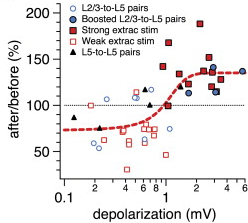
\includegraphics[width=0.5\textwidth]{./figures/sjoestroem_haeusser_plast_switch.jpg}
%\caption{From Sjöström and Häusser \cite{Sjoestroem_2006}: Somatic depolarization determines whether distal synapses undergo LTD or LTP upon stimulation.}
%\label{fig:ltp_switch}
%\end{figure}
%
%\subsection{Apical and Basal Compartments from an Information Theoretic Perspective}
%\subsubsection{Partial Information Decompositon}
%Recently, an information theoretic approach to characterizing multiple input channels called partial information decomposition (PID, see \cite{Williams_2010}) has been proposed as a framework for the understanding of the interplay between basal and apical inputs and its effects on information processing \cite{Wibral_2017}. In particular, Kay and Philips \cite{Kay_2019} analyzed the model proposed by Shai et al. \cite{Shai_2015} using PID. Roughly speaking, PID decomposes the total mutual information between neural input and output into three types of information: redundant, unique and synergistic information. In the case of a separation into apical and basal inputs, this would allow splitting the total information into a part that is provided by both input channels, unique information that is only provided by either apical or basal input, and information that is retrieved by means of the interaction between both input channels. Kay and Philips found that in the rate model by Shai et al., apical inputs provide very little unique information, but a a lot of synergistic information is present. Taken together, this is interpreted as apical input acting mostly ``modulatory"`rather than driving onto the neural output.
%
%\subsubsection{Interaction Information}
%Interaction information is an extension of mutual information to more than two variables \cite{McGill_1954}. For three random variables, the interaction information $I(X;Y;Z)$ is given by
%%%%%%%%%%%%%
%\begin{align}
%I(X;Y;Z) &= I(X;Y) - I(X;Y|Z) \\
%		&= I(X;Z) - I(X;Z|Y) \\
%		&= I(Y;Z) - I(Y;Z|X)
%\end{align}
%%%%%%%%%%%%%
%where e.g. $I(X ; Y)$ is the mutual information between $X$ and $Y$ and $I(X;Y|Z)$ is the conditional mutual information. The Latter is simply the expected value over $Z$ of the mutual information between the conditional probability distribution $P(X,Y|Z)$. Interpreting the given definition, interaction information quantifies if the knowledge of a third variable increases or decreases (on average) the mutual information between two other variables. Note that this quantity is not strictly positive. A positive sign of $I(X;Y;Z)$ indicates that $Z$ accounts for some of the correlation between $X$ and $Y$. This is a rather common case, e.g. if $X$ can be partly explained by $Z$. An example for negative interaction information would be a logical XOR gate $Z={\rm XOR}(X,Y)$, given that $X$ and $Y$ are independent binary variables. In this case, knowledge about the input $Y$ increases the mutual information between the input $X$ and the output $Z$.
%
%Interaction information can also be used to write the mutual information $I(Z;X,Y)$ between some hypothetical output function $Z=Z(X,Y)$ and a pair of input channels $X,Y$ as
%%%%%%%%%%%%
%\begin{equation}
%	I(Z;X,Y) = I(X;Z) + I(Y;Z) - I(X;Y;Z) \; .
%\end{equation}
%%%%%%%%%%%%
%That means, if interaction information is negative, more information about $Z$ is conveyed via $X,Y$ taken together than the sum of their individual information content about $Z$. In this scenario, $X,Y$ jointly provide some cooperative information that can not be retrieved by inspecting $X$ and $Y$ individually, in accordance with the interpretation of negative interaction information given above. In the other case, where interaction information is positive, the actual information provided by $X,Y$ is less than their individual information content. This could, for example indicate some form of redundancy, which, again is in accordance to the interpretation of positive interaction information previously given.
%
%
%\section{Possible Future Work}
%\begin{itemize}
%	\item As explained, plasticity in distal synapses does not follow a simple Hebbian learning scheme. Rather, experimental evidence suggests that the amount of somatic depolarization can change the sign of plasticity in distal synapses. Therefore, it might be worthwhile investigating the plasticity dynamics of a simple learning rule that incorporates these findings. Actually, if we combine a simple Hebbian learning rule $y_{\rm pre} \cdot y_{\rm post}$ with a multiplicative factor $(y_{\rm post}-\theta)$ that changes sign depending on postsynaptic activity, we essentially get a BCM-like rule:
%	\begin{equation}
%		\Delta w_{ij} \propto y_j y_i (y_i - \theta) \; .
%	\end{equation}
%	Such a type of learning rule has been studied extensively, however, has not been combined with a basal-distal compartment model.
%	
%	An alternative view on plasticity in distal dendrites would be to consider it a distinct synaptic integration zone. From this perspective, one could propose a Hebbian learning rule in which the postsynaptic term is just a function of the local sum of postsynaptic potentials. Similar to what we already found in Sect.~\ref{sect:dist_plast}, one would expect such a learning rule to align weights to the PC of all distal inputs.
%	
%	\item Interaction information is a relatively simple quantity that provides some insight into how two (or more) variables are linked with respect to their effect on a third variable. Fore example, in Fig.~\ref{fig:interact_inf}, this measure was numerically calculated for different input statistics of the two-compartment firing rate model given in \eqref{eq:simpl_prox_dist}. Interestingly, increasing the correlation between proximal and distal inputs reverses the direction of the gradient in the space of proximal and distal input variances. However, this should just serve as an exemplary calculation, and it remains to be discussed whether this measure could provide insight e.g. into how such non-linear compartment model differs in its information processing to a simple point neuron model. Furthermore, one could investigate the effects of plasticity onto this quantity.
%	\item Moldwin and Segev \cite{Moldwin_2020}: Perceptron learning in a biophysical compartment model.$\rightarrow$ maybe test these capabilities in our model?
%\end{itemize}
%\begin{figure}
%	\centering
%	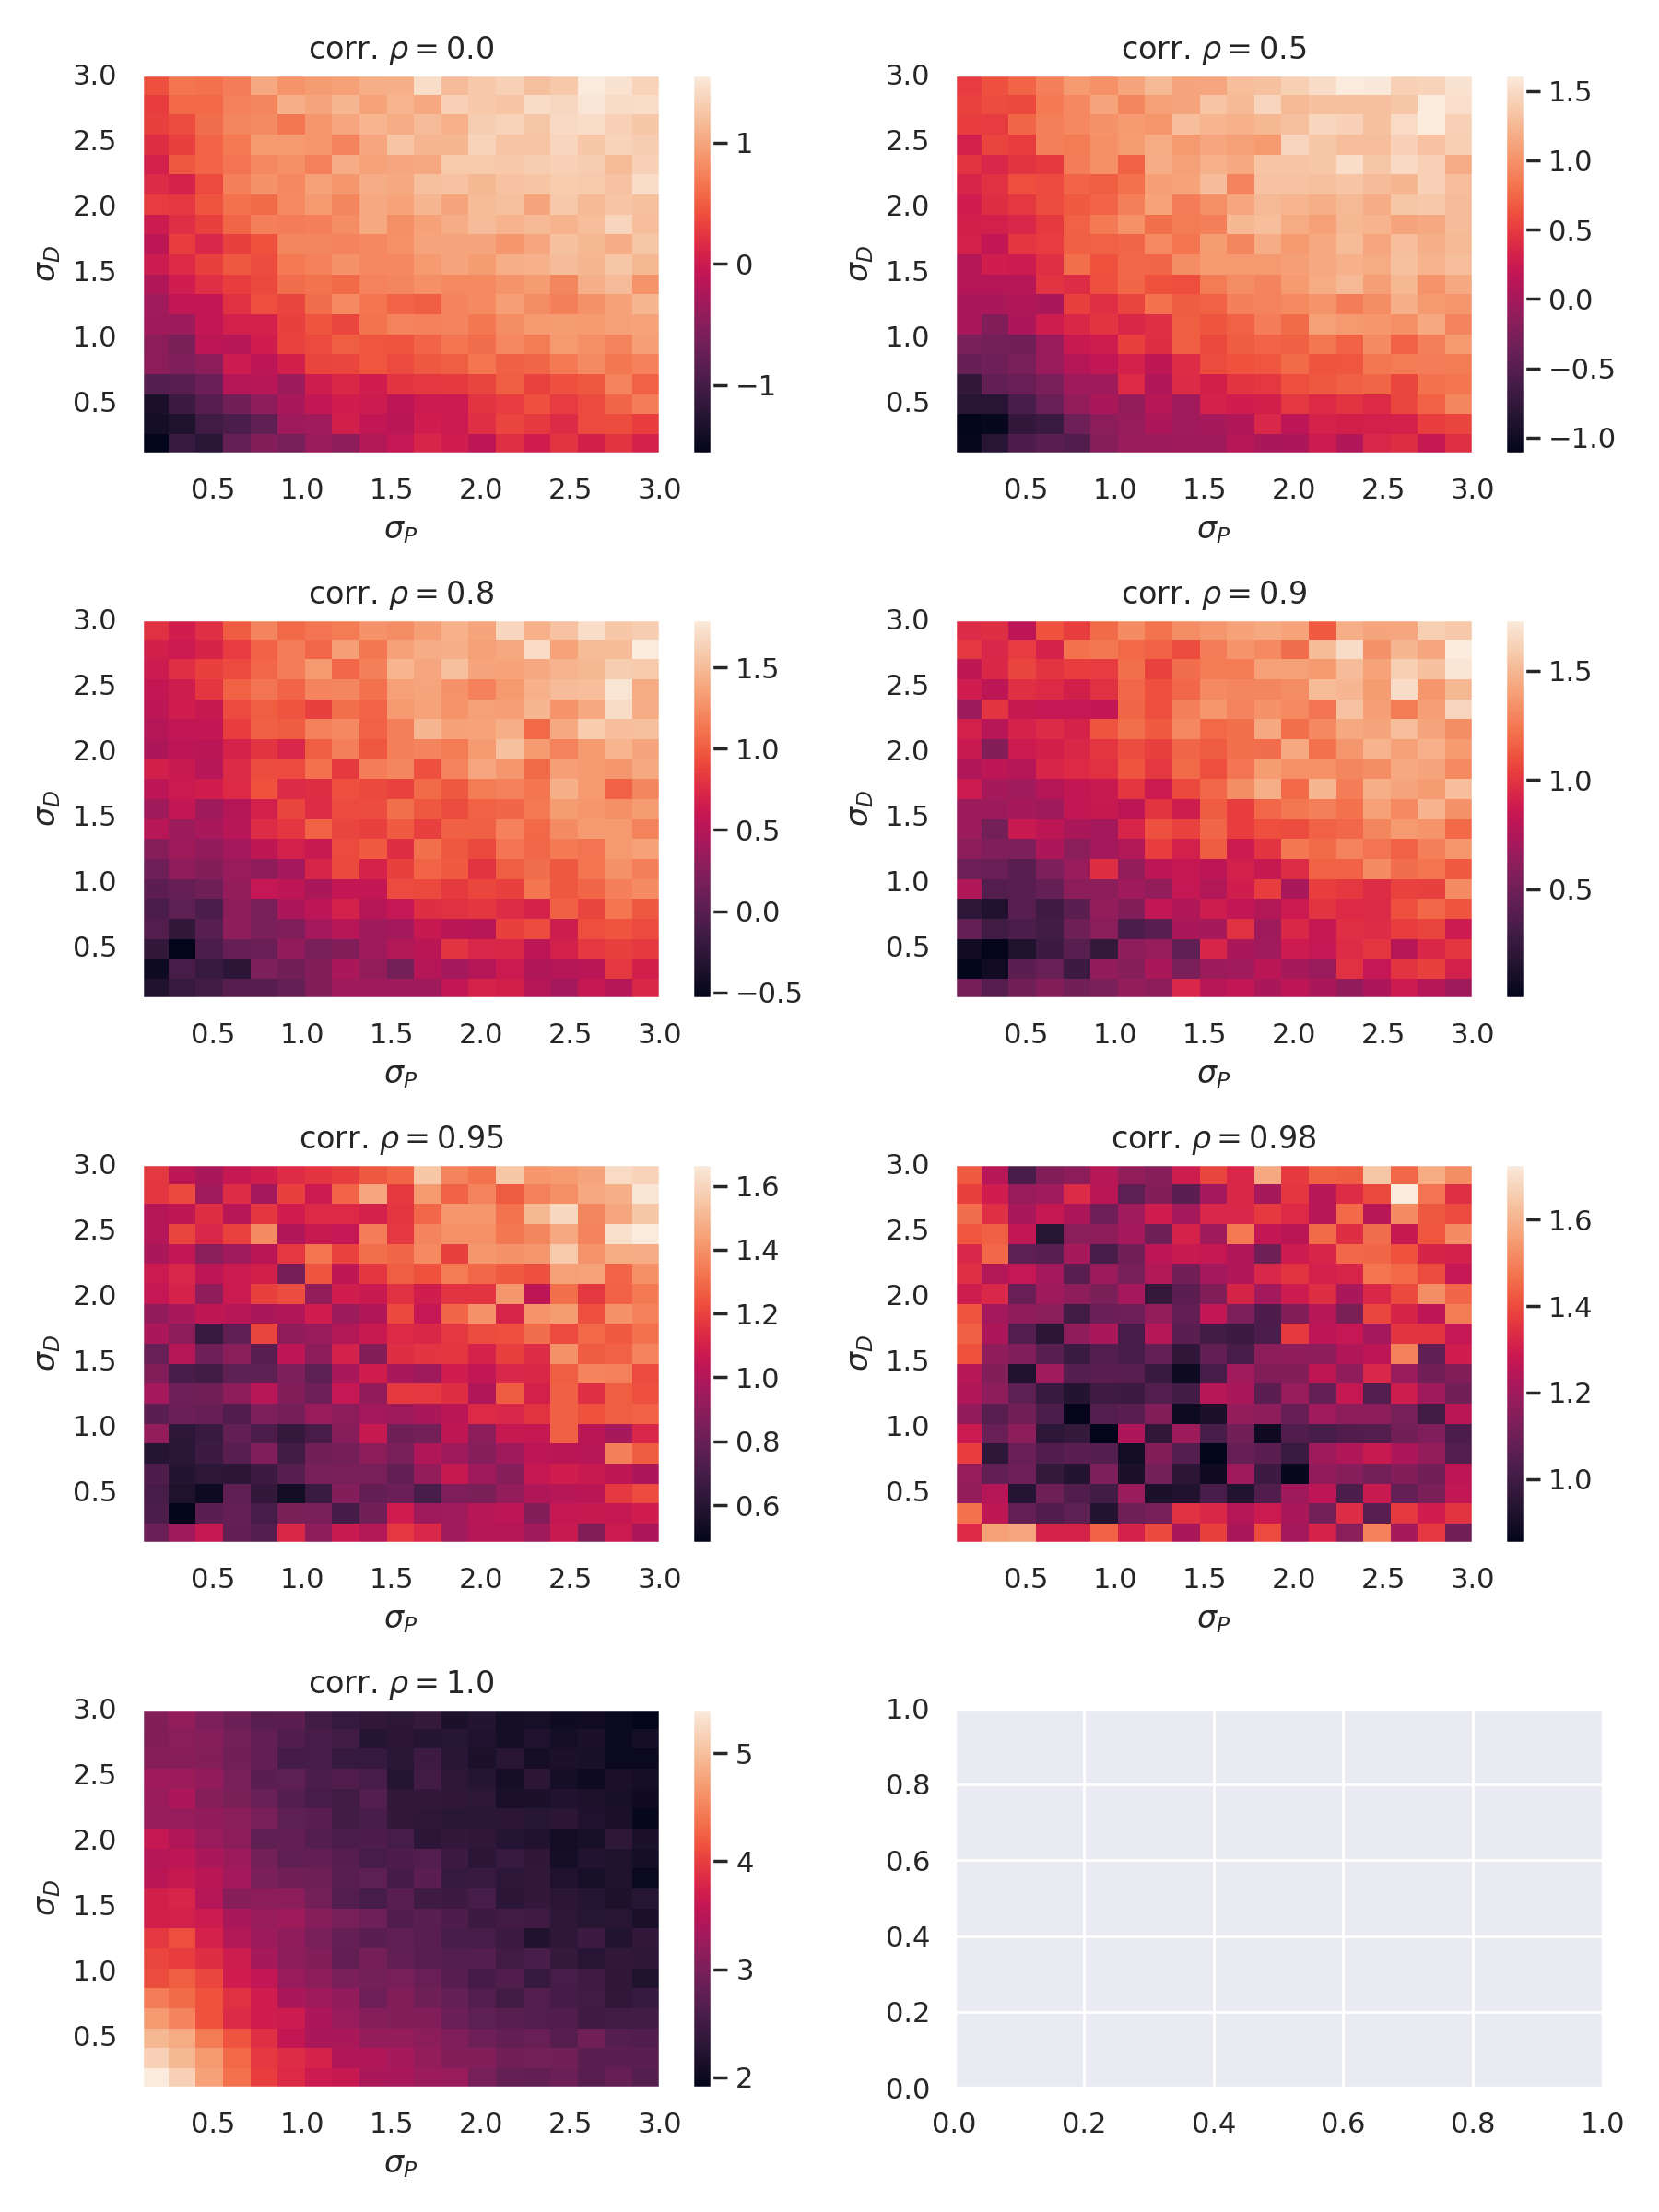
\includegraphics[width=\textwidth]{./figures/interaction_info_comp_mod.png}
%	\caption{Interaction information between and proximal input, distal input and the resulting firing rate of the compartment model given by \eqref{eq:simpl_prox_dist}. Inputs are Gaussian random variables with mean values of $0.5$ and standard deviations $\sigma_{\rm P}$ and $\sigma_{\rm D}$ respectively, and a correlation given by $\rho$.}
%	\label{fig:interact_inf}
%\end{figure}

  
\bibliographystyle{unsrt}
\bibliography{/home/fabian/work/lit_base.bib}
\end{document}